%!TEX TS-program = xelatex
%!TEX encoding = UTF-8 Unicode
\documentclass[16pt,a4paper]{article}

\usepackage{fontspec,xltxtra,xunicode}
\usepackage{array} % Word warp
\usepackage[table]{xcolor} % Zebra table
\usepackage[top=1.5in,bottom=1in,left=1.5in,right=1.5in]{geometry}

\usepackage{fancyhdr}
\pagestyle{fancy}
\lhead{การบ้านครั้งที่ 1}
\chead{}
\rhead{\bfseries โครงสร้างข้อมูลสำหรับจัดเก็บข้อมูลข่าว}
\lfoot{}
\cfoot{\thepage}
\rfoot{
    5870972621 นายสิทธิพงษ์ เหล่าโก้ก  \\
    วิศวกรรมซอฟต์แวร์ ภาคนอกเวลาราชการ
}

\setmainfont{TH Sarabun New}
\XeTeXlinebreaklocale 'th'
\XeTeXlinebreakskip = 0pt plus 1pt
\defaultfontfeatures{Scale=1.23}
\renewcommand{\baselinestretch}{1.2}
\newcolumntype{L}{>{\arraybackslash}m{3cm}}

\newcommand{\authorname}{นายสิทธิพงษ์ เหล่าโก้ก}
\newcommand{\dublincore}{Dublin Core}
\newcommand{\zebra}{\rowcolors{2}{white}{gray!10}}
\renewcommand{\refname}{อ้างอิง}
\renewcommand{\tablename}{ตาราง}
\renewcommand{\figurename}{รูปภาพ}

\newcommand{\thead}[1]{\multicolumn{1}{c}{\bfseries #1}}

\begin{document}

\noindent
\textbf{\underline{โจทย์}} จงนิยามโครงสร้างข้อมูลเพื่อจัดเก็บข่าวจากแหล่งข่าวที่แตกต่างกันซึ่งประกอบไปด้วยข้อมูล ได้แก่ สำนักข่าว วันที่เผยแพร่ หัวข้อข่าว เนื้อหาข่าว นักข่าว และประเภท เช่น ทั่วไป รายงานพิเศษ \\ \\
\textbf{\underline{คำตอบ}} การออกแบบโครงสร้างข้อมูลสำหรับแหล่งข่าวในครั้งนี้ได้นำรูปแบบการจัดเก็บโดยอ้างอิงจากโครงสร้างข้อมูล Dublin Core \cite{dublincore} ทั้ง 15 รายการ โดยคัดเลือกบางส่วนที่เกี่ยวข้อง ดังนี้ 

\begin{figure}[!htb]
    \centering
    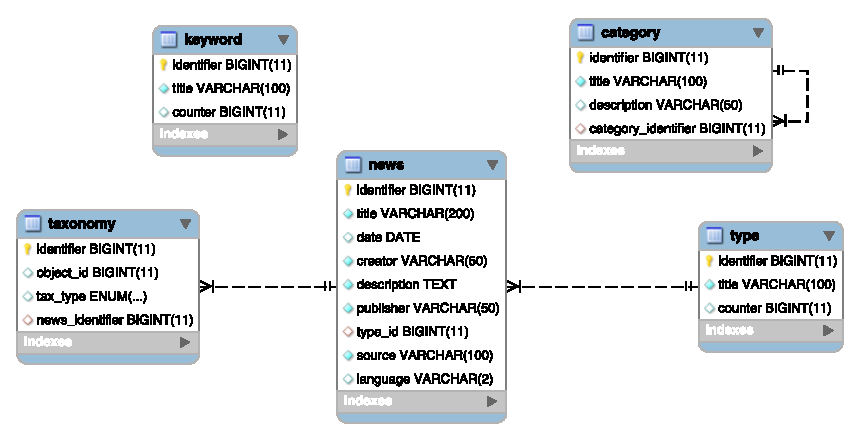
\includegraphics[width=0.75\textwidth]{fig/news-structure}
    \caption{ความสัมพันธ์ระหว่างตาราง}
    \label{fig:erdiagram}
\end{figure}

จาก\figurename \ref{fig:erdiagram} ข่าว (\textit{news} - \tablename\,\ref{tab:news}) สามารถระบุประเภทข่าวได้ 1 ประเภท ตามประเภทข่าวที่กำหนดไว้ (\textit{type} - \tablename\,\ref{tab:type}) 
และมีข้อมูลการแบ่งหมวดหมู่พร้อมจับคู่คำสำคัญ (\textit{taxonomy} - \tablename\,\ref{tab:taxonomy}) กันได้อย่างไม่จำกัดจำนวน ตามข้อมูลคำสำคัญ (\textit{keyword} - \tablename\,\ref{tab:keyword}) 
และหมวดหมู่ของข่าว (\textit{category} - \tablename\,\ref{tab:category}) ที่ได้กำหนดไว้ โดยที่หมวดหมู่ข่าวนั้นสามารถทำลำดับชั้นและกลุ่มของหมวดหมู่ได้ ซึ่งมีคำอธิบายโครงสร้างข้อมูลดังรายการด้านล่าง

\zebra
\begin{table}[!hbt]
    \caption{news: รายการข้อมูลสำหรับจัดเก็บข้อมูลข่าว}
    \label{tab:news}
    \centering
    \begin{tabular}{ | l | l | l | l | l | L | }
        \thead{ชื่อ}          & \thead{ประเภทข้อมูล}    & \thead{คีย์}            & \thead{คุณสมบัติ}    & \thead{ค่าเริ่มต้น}   & \thead{คำอธิบาย} \\ \hline
        \textit{identifier} & BIGINT(11)            & PK                    & auto\_increment   &                   & ชุดตัวเลขที่ไม่ซ้ำกันเพื่อใช้บ่งชี้ไปยังเนื้อข่าวที่จำเพาะเจาะจงได้\\ \hline
        \textit{title}      & VARCHAR(200)          &                       & NOT NULL          &                   & ข้อความสำหรับบันทึกหัวข้อข่าว \\ \hline
        \textit{date}       & DATE                  &                       &                   & CURRENT\_DATETIME & วันที่ที่เผยแพร่ข่าว โดยใช้รูปแบบ YYYY-MM-DD ตามที่ได้กำหนดไว้ในมาตรฐาน ISO 86013 \cite{iso8601} \\ \hline
        \textit{creator}    & VARCHAR(50)           &                       & NOT NULL          &                   & ชื่อนักข่าวผู้เขียนข่าวนี้ขึ้นมา \\ \hline
        \textit{description}& TEXT                  &                       & NOT NULL          &                   & เนื้อข่าว  \\ \hline
        \textit{publisher}  & VARCHAR(50)           &                       & NOT NULL          &                   & สำนักพิพม์  \\ \hline
        \textit{type\_id}   & BIGINT(11)            & FK (type.identifier)  &                   &                   & รหัสประเภทข่าว  \\ \hline
        \textit{source}     & VARCHAR(100)          &                       & NOT NULL          &                   & URL ของเนื้อหาข่าว \\ \hline
        \textit{language}   & VARCHAR(2)            &                       &                   & 'th'              & ตัวย่อของภาษา 2 ตัวอักษร อ้างตามมาตรฐาน ISO 639-1 \cite{iso639} \\ \hline
    \end{tabular}
\end{table}

\zebra
\begin{table}[!hbt]
    \caption{type: รายการข้อมูลสำหรับจัดเก็บประเภทข่าว}
    \label{tab:type}
    \centering
    \begin{tabular}{ | l | l | l | l | l | L | }
        \thead{ชื่อ}                  & \thead{ประเภทข้อมูล}    & \thead{คีย์}            & \thead{คุณสมบัติ}    & \thead{ค่าเริ่มต้น}   & \thead{คำอธิบาย} \\ \hline
        \textit{identifier}         & BIGINT(11)            & PK                    & auto\_increment   &                   & ชุดตัวเลขที่ไม่ซ้ำกันเพื่อใช้บ่งชี้ไปยังเนื้อข่าวที่จำเพาะเจาะจงได้ \\ \hline
        \textit{title}              & VARCHAR(100)          &                       & NOT NULL          &                   & คำสำคัญ \\ \hline
        \textit{counter}            & BIGINT(11)            &                       &                   & 0                 & จำนวนข่าวทั้งหมดที่จัดอยู่ในประเภทนี้ \\ \hline
    \end{tabular}
\end{table}

\zebra
\begin{table}[!hbt]
    \caption{keyword: รายการข้อมูลสำหรับจัดเก็บคำสำคัญ}
    \label{tab:keyword}
    \centering
    \begin{tabular}{ | l | l | l | l | l | L | }
        \thead{ชื่อ}                  & \thead{ประเภทข้อมูล}    & \thead{คีย์}            & \thead{คุณสมบัติ}    & \thead{ค่าเริ่มต้น}   & \thead{คำอธิบาย} \\ \hline
        \textit{identifier}         & BIGINT(11)            & PK                    & auto\_increment   &                   & ชุดตัวเลขที่ไม่ซ้ำกันเพื่อใช้บ่งชี้ไปยังเนื้อข่าวที่จำเพาะเจาะจงได้ \\ \hline
        \textit{title}              & VARCHAR(100)          &                       & NOT NULL          &                   & คำสำคัญ \\ \hline
        \textit{counter}            & BIGINT(11)            &                       &                   & 0                 & จำนวนข่าวที่เกี่ยวข้องกับคำสำคัญนี้ \\ \hline
    \end{tabular}
\end{table}

\zebra
\begin{table}[!hbt]
    \caption{category: รายการข้อมูลสำหรับจัดเก็บหมวดหมู่}
    \label{tab:category}
    \centering
    \begin{tabular}{ | l | l | l | l | l | L | }
        \thead{ชื่อ}                      & \thead{ประเภทข้อมูล}    & \thead{คีย์}        & \thead{คุณสมบัติ}    & \thead{ค่าเริ่มต้น}   & \thead{คำอธิบาย} \\ \hline
        \textit{identifier}             & BIGINT(11)            & PK                & auto\_increment   &                   & ชุดตัวเลขที่ไม่ซ้ำกันเพื่อใช้บ่งชี้ไปยังเนื้อข่าวที่จำเพาะเจาะจงได้ \\ \hline
        \textit{title}                  & VARCHAR(100)          &                   & NOT NULL          &                   & คำสำคัญ \\ \hline
        \textit{description}            & VARCHAR(50)           &                   &                   &                   & คำอธิบายหมวดหมู่ \\ \hline
        \textit{category\_identifier}   & BIGINT(11)            & FK (identifier)   &                   &                   & รหัสกลุ่มหลัก \\ \hline
    \end{tabular}
\end{table}

\zebra
\begin{table}[!hbt]
    \caption{taxonomy: รายการข้อมูลการจัดกลุ่มหมวดหมู่และคำสำคัญ}
    \label{tab:taxonomy}
    \centering
    \begin{tabular}{ | l | l | l | l | l | L | }
        \thead{ชื่อ}                  & \thead{ประเภทข้อมูล}            & \thead{คีย์}            & \thead{คุณสมบัติ}    & \thead{ค่าเริ่มต้น}   & \thead{คำอธิบาย} \\ \hline
        \textit{identifier}         & BIGINT(11)                    & PK                    & auto\_increment   &                   & ชุดตัวเลขที่ไม่ซ้ำกันเพื่อใช้บ่งชี้ไปยังเนื้อข่าวที่จำเพาะเจาะจงได้ \\ \hline
        \textit{object\_id}         & BIGINT(11)                    &                       & NOT NULL          &                   & รหัสข่าว \\ \hline
        \textit{tax\_type}          & enum('category', 'keyword')   &                       & NOT NULL          & 'keyword'         & ประเภทของการแบ่งหมวดหมู่ \\ \hline
        \textit{news\_identifier}   & BIGINT(11)                    & FK (News.identifier)  & NOT NULL          &                   & รหัสข่าว \\ \hline
    \end{tabular}
\end{table}

\newpage

\bibliography{references}
\bibliographystyle{plain}

\end{document}
